\documentclass[10pt,twocolumn]{article}
\usepackage{times}
\usepackage[pdftex]{graphicx}
\graphicspath{{./}{figs/}}

\begin{document}
\title{Artificial Life Creation Comparing Genetic Algorithms And Genetic Programming}
\author{Tom Cammann\\\\
Computer Science, cy004947@reading.ac.uk}
\date{}
\maketitle
\begin{abstract}
This report focuses on the generating artificial life through two distinct methods, genetic algorithms and genetic programming. The report describes the fundamentals of these two methodologies, compares and contrasts their differences in the creation of similar artificial life. The report outlines tools developed during this project to accomplish an effective comparison of these two methods. These include a method of visualising the artificial life and the environment it inhabits during its existence. The outcome of this project demonstrates how genetic programming requires more advanced programming but can lead to novel and emergent behaviour, in contrast to genetic algorithms which are much simpler and can better replicate biological processes that go on around us. 
\end{abstract}


\section{INTRODUCTION}

Artificial life or ALife is the study and implementation of systems that are simulations or replications of natural life.
These systems can be biochemical, mechanical, computer software and many other medium that supports the existence of structured self controlled information.
This report will be looking at software artificial life, or Soft ALife and how it can be implemented using evolutionary computation.
Evolutionary computation has been used for the creation of artificial life for many decades, REF + EXAMPLE.
Using evolutionary computation has many qualities that replicate naturally evolved life, and is one few computational methods known that can generate solutions to problems without human interaction.
Evolutionary computation has been applied to artificial life to generate life forms that can inhabit an environment and are 'solutions' to this environment.

\paragraph{}
Evolutionary computation generally works by generating a population of solutions to a problem, and then using this population to create a better next population that can solve the given problem better.
To create a better population crossover, mutation and selection are used in various forms to generate a fitter population.
Each of these populations is referred to as a generation.
Each member in the population is a solution to the problem, however these solutions do not have to be correct, and are often close to correct before many generations have passed.
Each member of the population is assigned a fitness value to correspond with how close the solution is to correct, or how effective the solution is.
In the Context of artificial life this fitness value may correspond to how well the life form survives in a given environment.

% why are we comparing these 2 methods
\paragraph{}
The purpose of this investigation is to compare and contrast the usage of genetic algorithms and genetic programming in the creation of artificial life. Genetic programming first became prevelvant in the early 1990 after Koza used used GP to solve ??? ~\cite{Koza90}. After the advancements made by Koza many applications for GP emerged and one of the earlier appications was in ALife. Before these advancements GA was the primary method for generating ALife.

However these two have very different implementations and usage, this report will investigate the usage of both in the context of artificial life creation. 
% Genetic programming can generate unique solutions, unrestrained, GA more restrained. 

\paragraph{}
%how we compare them



\section{GENETIC ALGORITHMS}

Genetic algorithms were first designed and implemented by ??? in ??? when ???.

The general form of a genetic algorithm uses genes to represent parameters inside a program.
These parameters effect the running of a program.
These genes were historically represented in binary form, however more modern implementations can use any value as a gene, from programming objects to double floating point numbers.
These genes must be able to mutate, this is easy to understand when using binary number, to mutate a binary number you flip one bit in the gene sequence. 

\subsection{POPULATION REPRESENTATION}
In genetic algorithms each member of the population (or candidate solution) is represented by a list or string of values.
Each value represents a parameter that will be used in the solution.
The value could represent the number of iterations of a loop or represent a operator in a sum.
Traditionally binary numbers strings were used to represent a member of the population.
This was because of the ease of which this could be manipulated by computers and the simplicity mutations could be achieved.
To mutate a binary string a bit can be flipped.
This can work in most situations however it soon becomes apparent that this cannot useful in all situations.
%Fix and show formula? Find solutin.
If numbers are being represented in binary strings the most significant bit is at start of the string, if this is flipped then the number will change by a factor of ???.


\subsection{MUTATION}
In genetic algorithms mutation occurs on a per gene basis. If a mutation for a population member is needed then a gene in that~\cite{j1}. 

%better title needed!!!
%Section about how this project uses GA
\subsection{USAGE IN THIS}

\section{GENETIC PROGRAMMING}
%intro to gp
Genetic programming is one of the newest forms of evolutionary computing. 
%different ways


\subsection{POPULATION REPRESENTATION}
%obv

\subsection{MUTATION}
%asdsss
\section{DEVELOPMENT}

This project was written in Java programming language and was developed on serveral operating systems during its life time. Java was chosen because of
a strong prior intimate knowledge of the language and because of the libraries available to develop with. The evolutionary computation libraries which
this project are based also use Java, this made interfacing with them very easy. Another reason Java was chosen was because of the graphical user interface 
programming libraries supplied as standard in Java. Having prior knowledge of these also meant that developing a visual format for the simulation could be 
accomplished. 

Along with using Java for development several other tools were used these were Eclipse, Maven and Git. Eclipse is a Intergrated Development Enviroment or IDE which
provides the user with an interface with faster programming and debugging ablities than are available as standard. This meant faster development. Maven was used a build tool to manage dependcies and build jar files for running the application that contains the simulations. Using this made it easy to develop on any computer, as managing the depenecies necessary for the program done all by Maven. Git was used as the the version control system for this project, this was only adopted towards the end of the project as it became more necessary to manage versions and have a reliable branching system. This project was hosted on GitHub.com which 
meant that development could quickly begin from any location with git available. 

\subsection{DESIGN AND ARCHITECTURE}


\section{SIMULATION}
To evaluate a common artificial life form a simulation environment has been created.
This environment is a 2D arena where a life form must continue to consume food to survive, the more food the life form consumes the fitter the  

The underlying genetic and evolutionary computations were completed on a Java framework called JGAP (Java Genetic Algorithms Package).
This package provides a tried and very well tested method for using genetic algorithms in Java, while also providing the 
ability to extend the package and use the package to fit into this projects needs. The package was tested several times before usage
and simple life forms were developed to ensure this package was appropriate. Other packages such as %TODO other packages
were used but found to be lacking extendibility and documentation. JGAP has very good documentation, which meant that extending
the package and adapting the package to this projects needs was even easier.

JGAP provides two general over arching algorithm frameworks to work with, genetic algorithms and genetic programming. However
the package does not provide any high level interfaces between the genetic algorithms side and the genetic programming side. A 
lot of development during this project was focused on developing a framework for evolution that could incorporate both GAs and GPs developed
using JGAP. 

Visualising both the GP and GA in the life form meant developing an abstract way of representing the state of the life form. This was done
through an abstract class called ALife. This abstract class provided a high level interface for other objects to read (and modify if necessary)
the state of the life form. The abstract class contained many of the variables for the life form and the setting and getting functions 
associated with them. 

\subsection{LIFE}

This project has modeled life on upon a fairly simple scenario, with only a few state variables. The states that this life form
can control are: its position on the map, its orientation and its energy level. Its position can be changed by moving forward, these 
forms can only move in the direction they are facing. The can modify their orientation by moving either right or left of where they 
are currently facing. They can also change their energy, however this is more passive than active. The life form's energy will
deplete during its life based on how much it moves and what actions it takes. However its energy can be increased by consuming a 
resource, this resource will contain a number of calories which can be converted into energy. This conversion rate is variable
depending on the life forms parameters. 

The simulation is split up into frames, during each frame the life form has a chance to move and interact with the environment. If their
are multiple life forms in the environment then each life form in turn will get a chance to interact during this frame. These frames are
meant to represent time for the life forms, it has been slightly simplified to be an amount of time a life form can move forward or interact in another way. Only one 'major' interaction can be completed per frame. These include moving, consuming a resource and turning.

To survive in an environment the life form must keep its energy above zero for the duration of the simulation, if the life forms energy
drops to zero or below then the life form will be assumed deceased and can no longer make any more interactions with its environment. A simulation can have indefinite run time and how long the life form can survive will depend on its fitness and availability of resources for energy.

When a life form needs to be tested for fitness it is added to a map, and the life form is asked to make an action for every frame. The life form starts out
with a nominal energy value, so that it does not die at the start of the simulation. A fit life form will then make intelligent actions and move towards resources
that it can consume to increase its energy level. The fitness of the life forms is accessed usually assessed by its energy level at the end of the simulation. 


\subsection{MAP}

The environment that the life forms exist on during the simulations are referred to as maps. These maps are two dimensional and can vary in size.
The size of the map can be set at run time and can also be set to dynamically change during a run if necessary. The map also holds references
to the resources contained in the environment. The map is split up into cells which form a 2D grid for which the life forms can inhabite. 

Generally for evolving good fit life forms a unique map is generated for each simulation. This creates an enviroment in the life form has not
seen before and has not adapted to before. This means that the fit life forms are the ones which will be able to adapt to any give situation
and still be able to consume and interact with their environment. Each time a map is generated a new set of resources is generated with different
positions on the map and different calorie values. If a static map is used, with the same positions of resources for each run, a very specialised 
life form can evolve but as soon as this life form is transposed into another environment this life form is very unfit.

The resources generated for each map are randomly placed, with random calorific values. Only one resource can ocupy a cell on the map, each resoruce also has
a type which can be checked by the life form. If a life form is on top of a resource, i.e. it is in the same cell then the life form can consume a resource. 
T 

%talking about how the project framework
%how a frame to accommodate genetic programming and GA
\subsection{EVOLUTIONARY FRAMEWORK}
To investigate and compare these two algorithms %? algorithms??%
a framework to accommodate both algorithms was produced. This framework had to allow comparison of the effectiveness and fitness of the life forms evolved, efficency of the 
evolutionary computations in generating a fit life form and the correctness of the solutions generated. To enable all these things an abstract framework had 
to be developed to allow comparison without respect to the algorithm that was used. This first accomplished by visualising members of the population and 
manually inspecting the fitest life form of each generation. 


\subsection{VISUALISATION}
Visualisation of the solutions (or life forms) produced by the algorithms was key
to understanding the differences produced in the life forms between the two algorithms. A visualisation of the map and life form
was developed early on. The visualisation was developed using the model view controller architecture,
which meant that the map and the life form were completely detached from the visualisation.
The life form was made abstract by using an abstract class which contains the basic variables need for the life
form and some simple functions to get and set these variables. These include the life forms position, orientation
and energy level. The visualisation renders the 2D map with resources on, with the cell size depending on the attributes selected at runtime. The frame speed can
adjusted during the visualisation, but is default set to 5 frames per second. The visualisation itself is contained within the visualisation window. This window
provides access to the visualistation such as start, stopping and restarting the simualtion.


The visualisation has also been used to debug the life forms produced, to find errors in the project code which the life forms have ended up exploiting. An example
of this was during early development their existed a bug that cause the life form to stop decrementing its energy when it got to a map corner. When the simulation
was run with this bug in the life forms would evolve to find the corners of the map as they could get stuck their and never die. These life forms were not that fit 
as they usually only had a fitness value that was around their starting energy.

Later in development other features were added to the visulisation window. One of these features was the ability to import and export maps for the life forms to be
tested out on. A previously generated made could be loaded and the life form could be assessed on how it dealt with the that particular map. Producing this ablity meant that it would be easier to compare life forms, understanding exactly how they interacted with the same environment.
Another feature that was added was the ablitity to run the simulation frame by frame. The user can pause the simulation and step through the simulation, this again provides another method of fully understanding how a life form interacts with the enviroment. 
Along with the ablities to interact with the simulation was the ablitity to access information on the current life form, such as its genetic make what generation
and run time parameters were involved with its creation.



\begin{figure} [ht]
\centering
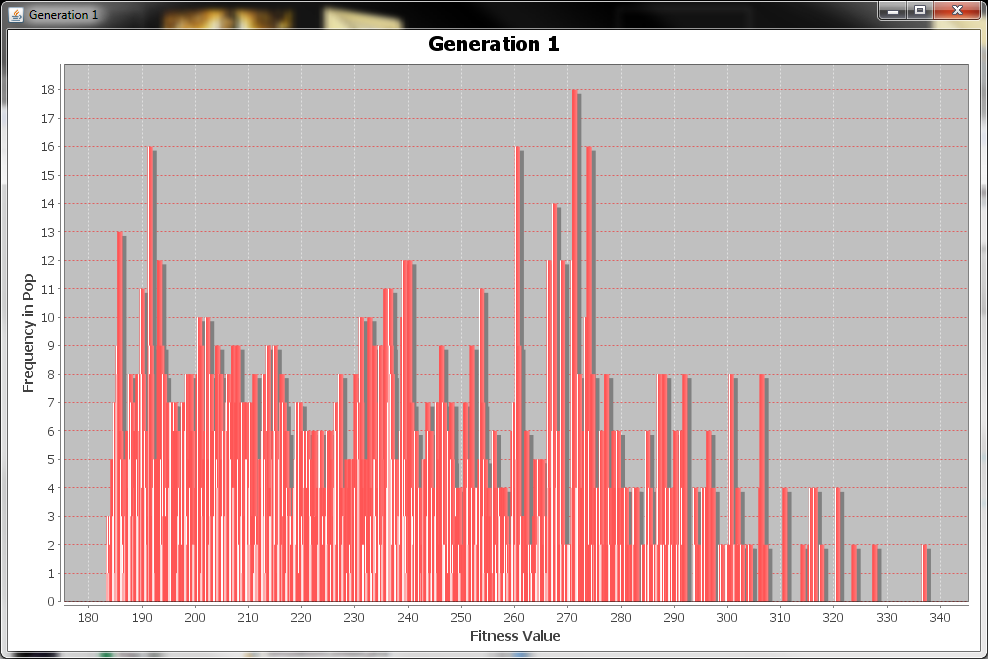
\includegraphics[scale = 0.25]{gen1-2500.png}
\caption{My figure}
\label{the-label-for-cross-referencing}
\end{figure}


\bibliographystyle{plain}
\bibliography{disseration}

\end{document}
